\newcommand{\source}[1]{\caption*{Source: {#1}} }

\section{Verwandte Arbeiten}\raggedbottom

\subsection{Semantische Segmentierung im medizinischen Bereich}

\subsubsection{Semantische Segmentierung}

Die semantische Segmentierung erfolgt in drei Schritten:

Klassifizierung: Klassifizierung eines bestimmten Objekts im Bild.
Lokalisieren: Auffinden des Objekts und Zeichnen eines Begrenzungsrahmens um das Objekt.

Segmentierung: Gruppierung der Pixel in einem lokalisierten Bild durch Erstellung einer Segmentierungsmaske.

Im Wesentlichen kann man die Aufgabe der semantischen Segmentierung als Klassifizierung einer bestimmten Bildklasse und deren Abgrenzung von den übrigen Bildklassen durch Überlagerung mit einer Segmentierungsmaske bezeichnen.

Allgemein kann man es sich auch als Klassifizierung von Bildern auf Pixelebene vorstellen.

\subsubsection{Medizinischer Bereich}

Die medizinische Bildgebung umfasst viele Kategorien, von 2- bzw. 3 dimensionalen MRT Scans des Herzens, Gehirns und des Magen-Darm Trakts, 2 dimensionalen Röntgen Bildern sowie Ausschnitte aus der Videoendoskopie.

Bereits in den 90er Jahren wurde sich mit mit Segmentierungsarchitekturen auseinandergesetzt und baselines geschaffen. Zu dieser Zeit lieferten Methoden im Bereich \glqq Pattern recogniction\grqq die besten Ergebnisse. Die Autoren legten viel Wert auf preprocessing der Daten und werteten die zu jener Zeit besten Modelle aus. Es handelte sich um einen Feature basierten Ansatz, es wurden Algorithmen wie
\href{https://en.wikipedia.org/wiki/K-nearest_neighbors_algorithm}{kNN},
\href{https://en.wikipedia.org/wiki/Maximum_likelihood_estimation}{Maximum Likelihood} und
\href{https://en.wikipedia.org/wiki/Eigenvalues_and_eigenvectors}{Characteristic vector} getestet.

Trotz aller Bemühungen wiesen die Modelle nur eine Accuracy von 3\% bis 34\% auf. \citep{Clarke:Mri1995}

Jedoch waren die Autoren davon überzeugt, dass Segmentierung eine wichtige Rolle im Beriech der Verarbeitung von MRT Daten darstellen wird und mit wachsender Akzeptanz auf klinischer Seite sowie dem technischen Fortschritt der Hochleistungsrechner es in Zukunft möglich sein wird, akkurate Segmentierungen von MRT Scans im Livebetrieb vorzunehmen.

\newpage

\subsection{Deep Learning-Techniken für die Segmentierung medizinischer Bilder:
Errungenschaften und Herausforderungen}

Dank der immensen Verbesserung der Rechenleistung der Hardwarecomponenten wurde das Thema Deep Learning immer interessanter und gehört heutzutage zur standard Herangehensweise. Architekturen wie das U-Net Modell \citep{U-Net} haben sich hierbei besonders bewiesen und wurden mit den Jahren nach der Veröffentlichung in 2015 stetig erweitert, so dass es für viele verschiedene (medizinische) Bereiche Architekturen vorliegen, die auf die jeweiligen Problemstellungen angepasst wurden, jedoch trotzdem Anwendung auf ähnlichen Gebieten finden können \citep{Hesamian}

\subsection{Intelligentes Zuschneiden des Inputs}

Dimitrios G. Zaridis et al. \citep{SmartCrop} haben sich ebenfalls mit verschiedenen State of the Art U-Net Architekturen auseinandergesetzt und jene als Baseline für ihre Arbeit genutzt. Trotz der beachtlichen Leistung, die die Modelle liefern, sind sie der Meinung dass noch Verbesserungspotential vorhanden ist.

Sie fanden heraus, dass das Vorhandensein eines Klassenungleichgewichts, wo der Anteil der Hintergrundpixel dem Anteil des zu segmentierenden Organs überwiegt zu Problemen führt. Mithilfe eines Deep Learning Modells haben die Autoren es geschafft, dieses Klassenungleichgewicht zu reduzieren, in dem das Neuronale Netzwerk die gesuchten Organe lokalisiert, das Originalbild zuschneidet und am Ende das Verhältnis von Vorder- und Hintergrundpixeln normalisiert. Dies führte bei allen gängigen Deep Learning Netzwerken zu erheblichen Verbesserung im Bezug des Dice-Scores. U-Net+ und ResU-Net++ wiesen mithilfe diese Verbesserungen von bis zu 8\% auf.

\section{Grundlagen}\raggedbottom

\subsection{Magen-Darmtrakt}

Um die Daten zu verstehen und Erkentnisse aus den Ergebnissen zu gewinnen, ist es wichtig ein Grundverständnis für den Bereich des Körpers zu haben, den unsere Daten beschreiben. Wir interessieren uns in unserem Fall für den Dick- bzw. Dünndarm sowie den Magen. Hierbei liegt die Herausforderung, dass je nach Ernährungsverhalten, Schlafposition, anderen Krankheiten und Verdauung die Position der Organe stark (bzw. stärker als andere) variieren kann. Mithilfe der Grafik kann man sich ein Bild vom groben Aufbau machen. \autoref{magen-darm-trakt}

\begin{figure}[htb]
	\begin{center}
		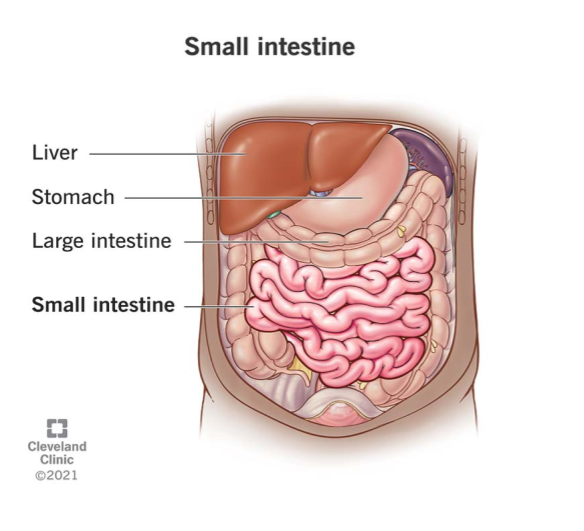
\includegraphics[width=450pt]{bilder/intestines}
		\caption{Magen-Darm Trakt}\label{magen-darm-trakt}
	\end{center}
\end{figure}

\begin{figure}[htb]
	\begin{center}
		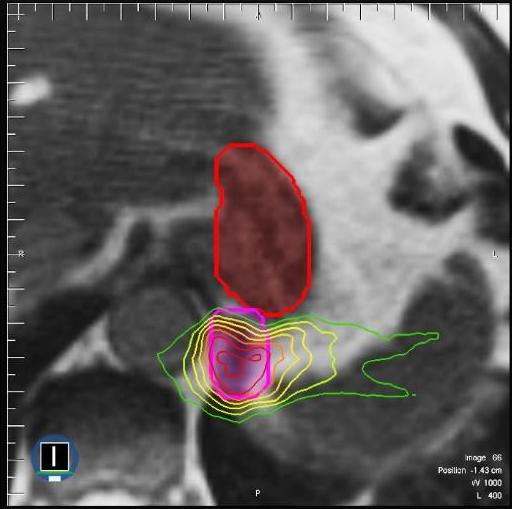
\includegraphics[width=450pt]{bilder/magen-mrt}
		\caption{Beispiel MRT des Magen-Darm Traks. Zu sehen ist der Magen (rot) und der Tumor (pink) sowie die verabreichte Strahlendosis. Die Strahlenintensivität werden durch den Regenbogen der Umrisse dargestellt, wobei höhere Dosen rot und niedrigere Dosen grün dargestellt werden.}\label{magen-mrt}
	\end{center}
\end{figure}

\subsection{U-Net}
% CNN, Convolution, Maxpooling oder ReLu erklären?

U-Net wurde im Jahr 2015 von Olag Ronneberger et al. \citep{U-Net} vorgestellt als Segmentierungsarchitektur für den biomedizinischem Bereich und bildet die Baseline dieser Arbeit. Neu in der Herangehensweise ist der Encoder-Decoder Part, die dem Netzwerk ermöglicht räumliche Merkmale anzutrainieren.
Klassisch handelt es sich beim Encoder um ein
\href{https://en.wikipedia.org/wiki/Convolutional_neural_network}{Convolutional Neural Network}, bestehend es aus 5 bis 6 \glqq downsampling\grqq Schichten und der gleichen Menge an \glqq upsampling\grqq Schichten im Decoder-part. 

Eine \glqq downsample\grqq  Operation besteht zum einen aus einer
\glqq \href{https://en.wikipedia.org/wiki/Convolution}{Convolution Operation}\grqq
sowie einer
\glqq \href{https://computersciencewiki.org/index.php/Max-pooling_/_Pooling}{Max Pooling}\grqq
an deren Ende jeweils eine
 \glqq \href{https://deepai.org/machine-learning-glossary-and-terms/relu}{ReLu}\grqq
 Aktivierungsfunktion zum Einsatz kommt. In diesem Schritt lernt das Modell Eigenschaften auf Pixelebene, wie zum Beispiel Formen, Ecken, Kanten. Hierbei halbieren sich die Eingabedimensionen und die Tiefe des Bildes wird erhöht. Veranschaulicht kann man sagen, dass das Modell das \glqq Was\grqq lernt, was im Bild zu sehen ist. \citep{Con97} Zur Semantischen Segmentierung fehlt dann nur noch das  \glqq Wo\grqq, hierbei wird das Zusammenspiel von En- und Decoder deutlich.

Im Decoder wird das Bild wieder auf seine ursprüngliche Größe mittels 
\glqq \href{https://en.wikipedia.org/wiki/Deconvolution}{Transpose Convolution operations}\grqq  
gebracht. Hier ersetzt die transponier Operation die Maxpooling Operation (vergleich Grafik). Dieser Part erlaubt dem Modell das lokalisieren der zuvor gelernten Eigenschaften. Output ist eine Maske, bestehend aus Nullen und Einsen, die der Eingabegröße gleicht und bestenfalls den Wert Eins an der Stelle des gesuchten Organs enthält.

\begin{figure}[htb]
	\begin{center}
		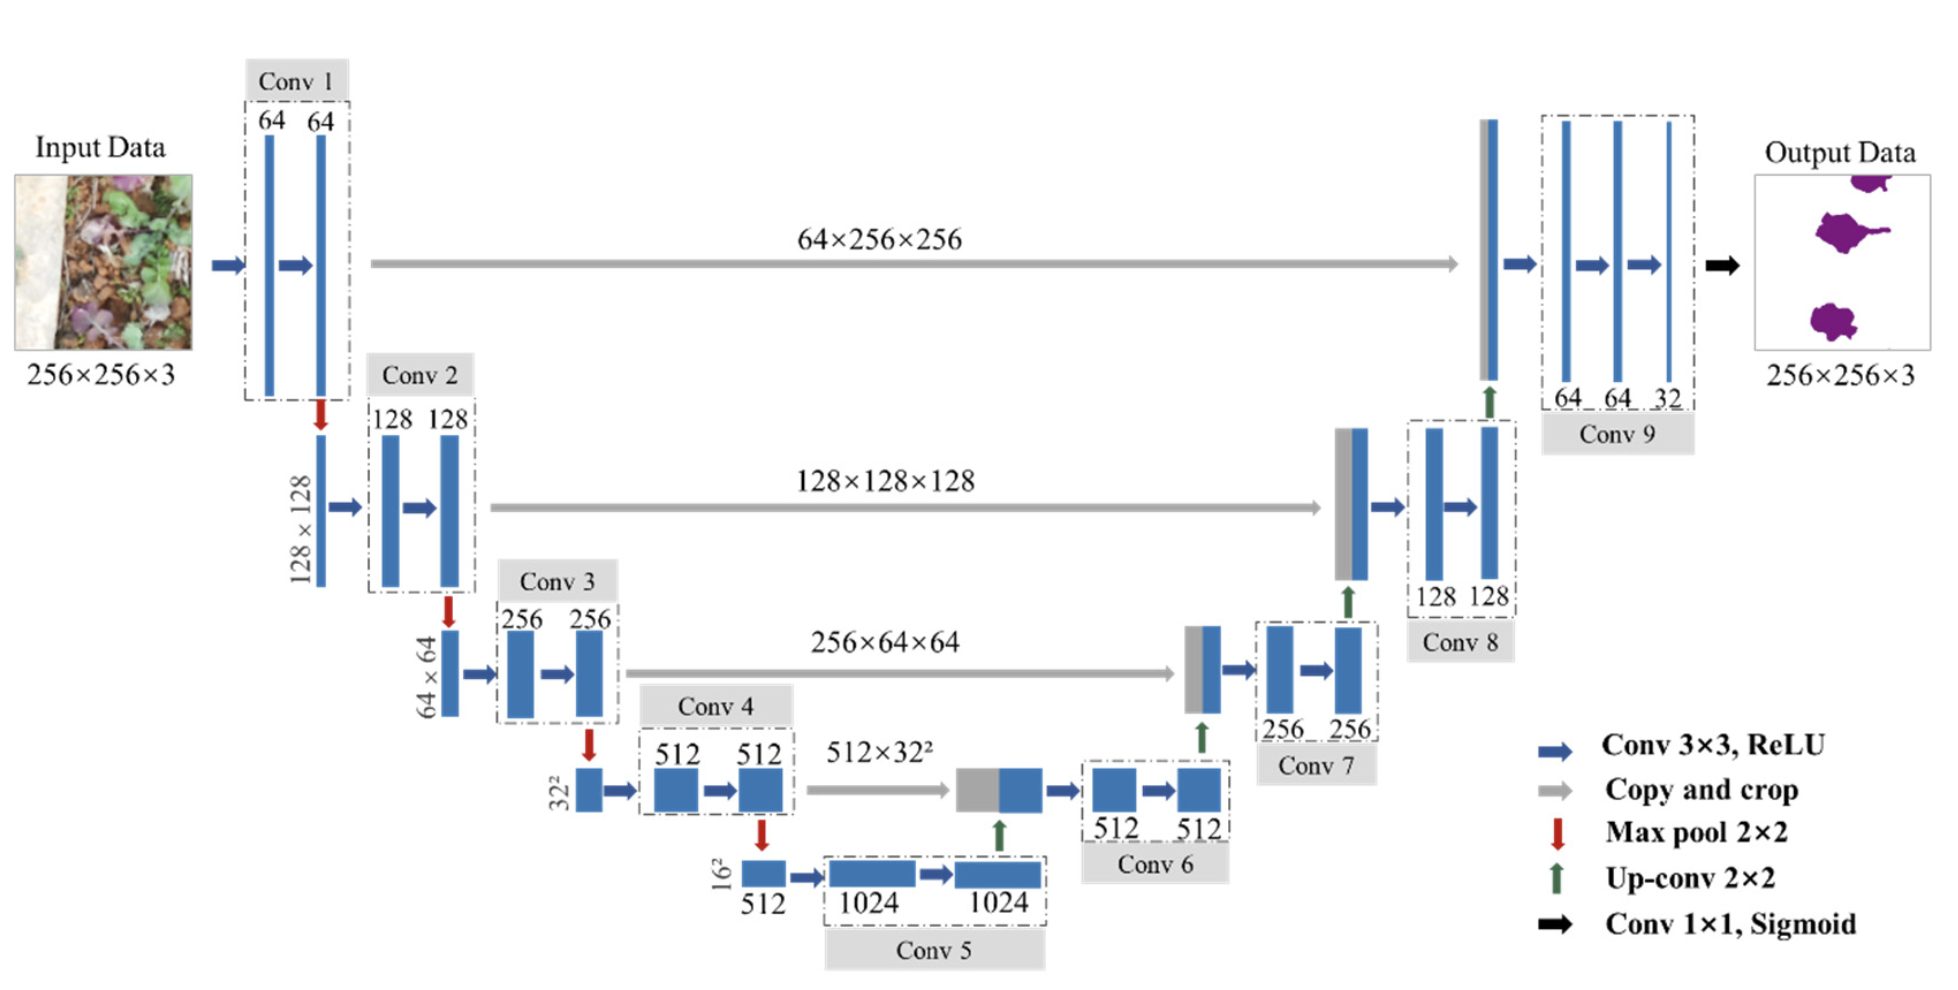
\includegraphics[width=300pt, angle=270]{bilder/u-net-architecture}
		\caption{U-Net Architektur}\label{Fig:unet-diagram}
	\end{center}
\end{figure}


\subsection{Encoder 1}
Eventuell

\subsection{Kaggle}

Diese Arbeit baut auf der 
\href{https://www.kaggle.com/competitions/uw-madison-gi-tract-image-segmentation/overview/description}{UW-Madison GI Tract Image Segmentation}
Challenge auf, die von der \glqq University of Wisconsin Carbone Cancer Center Pancreas Pilot Research Grant \grqq organisiert wurde und von denen die Daten auch bereitgestellt wurden.

Evaluiert wurden die Ergebnisse mit einer Gewichtung von 0.4 des Dice-Koeffizienten  (\autoref{ssec:dc}) sowie 0.6 der Hausdorff-Metrik (\autoref{ssec:hdorff}) auf unbekannten Testdaten.


\section{Methodik}\raggedbottom

\subsection{Datenanalyse}

Im Folgenden beziehen sich die Werte {X} immer auf auf die Vorhersage und {Y} auf die Groundtruth.

\begin{table}[H]
	\begin{center}
	        \small
	        \setlength\tabcolsep{2pt}
		\begin{tabular}{|c|c|c|c|c|c|c|c|c|}
			\hline
			Index  & ID & Class & Segmentation \\
			\hline \hline
			1     & case134\textunderscore day0\textunderscore slice\textunderscore 0085 	& large\textunderscore bowel 	&  NaN  \\
			2     & case134\textunderscore day0\textunderscore slice\textunderscore 0085 	& small\textunderscore bowel 	&  41591 5 41599 7 41949 27 ...  \\
			3     & case134\textunderscore day0\textunderscore slice\textunderscore 0085 	& stomach 	&  NaN \\
			4     & case123\textunderscore day0\textunderscore slice\textunderscore 0001 	& large\textunderscore bowel 	&  35223 6 74352 7 32312 12 ...   \\
			5     & case123\textunderscore day0\textunderscore slice\textunderscore 0001 	& small\textunderscore bowel 	&  63432 5 12354 7 41949 12 ...  \\
			6     & case123\textunderscore day0\textunderscore slice\textunderscore 0001 	& stomach 	&  NaN \\
			\hline
		\end{tabular}
		\caption{Beispieldaten für zwei Slices}\label{tabelle_daten}
	\end{center}
\end{table}

Der Datensatz besteht aus 115 488 Zeilen und enthält drei features: ID, Klasse und einem Run-lenght codierten String, der die Maske enthält. \autoref{tabelle_daten}. Jeder ID sind drei Zeilen gewidmet, jeweils für die drei Klassen: small\textunderscore bowel, large\textunderscore bowel und stomach. Zu jeder ID existiert ein graustufen Bild, welche sich im train Ordner befinden, Ein Beispiel der Ordnerhierarchie kann man hier sehen \autoref{Fig:train-data}.

input\textbackslash uw-madison-gi-tract-image-segmentation\textbackslash train\textbackslash case101\textbackslash \\case101\textunderscore
day20\textbackslash scans\textbackslash slice\textunderscore 0001\textunderscore 266\textunderscore 266\textunderscore 1.50\textunderscore 1.50.png

\begin{figure}[htb]
	\begin{center}
		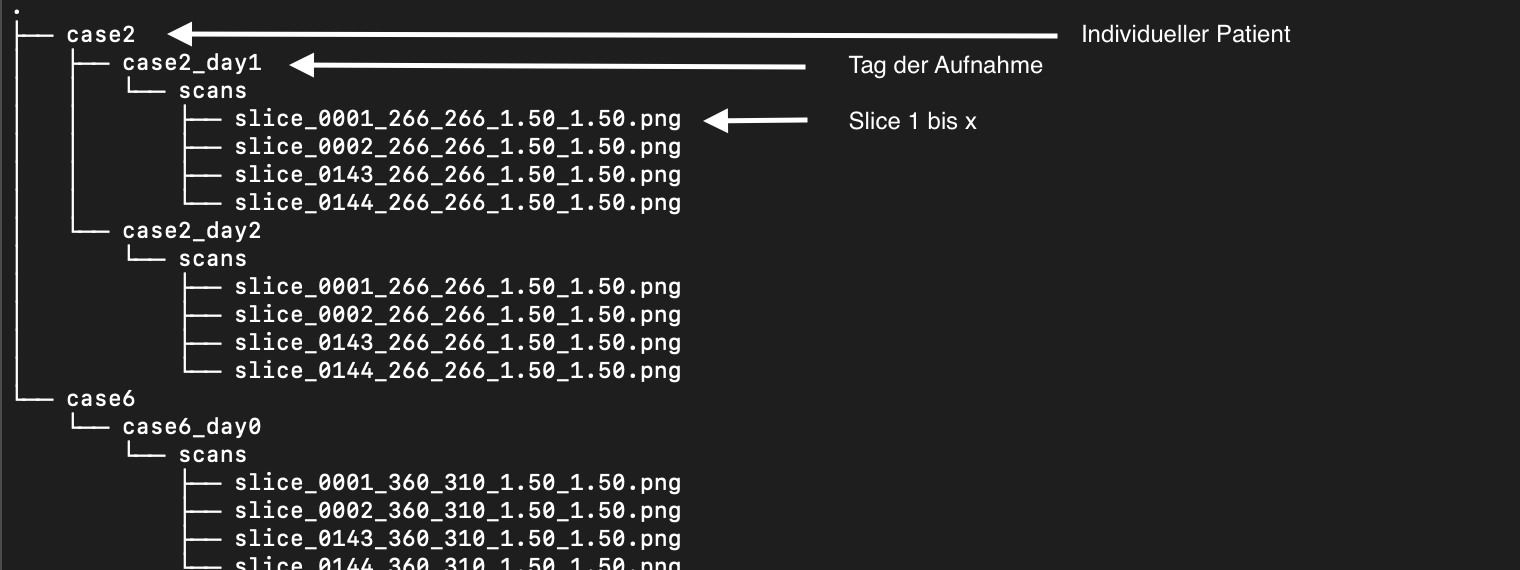
\includegraphics[width=450pt]{bilder/data_tree}
		\caption{Trainingsdaten Hierachie}\label{Fig:train-data}
	\end{center}
\end{figure}

Jedes slice enthält vier Zahlen (z.B. 266\textunderscore 266\textunderscore 1.50\textunderscore 1.50.png), die ersten beiden stehen für die Auflösung des Bildes und die letzten beiden für den physischen Abstand der Pixel. Der Großteil der Aufnahmen stammt von Tag null oder Tag eins \autoref{Fig:slice_per_day} und die durchschnittliche Anzahl an Bildern pro Fall beträgt X.

Beim betrachten der Verteilung der Segmentierungen fällt auf, dass das Vorkommen für jede Klasse stark variiert, am häufigsten sind gar keine segmentierten Slices. \autoref{Fig:klassenverteilung}.

\begin{figure}[htb]
	\begin{center}
		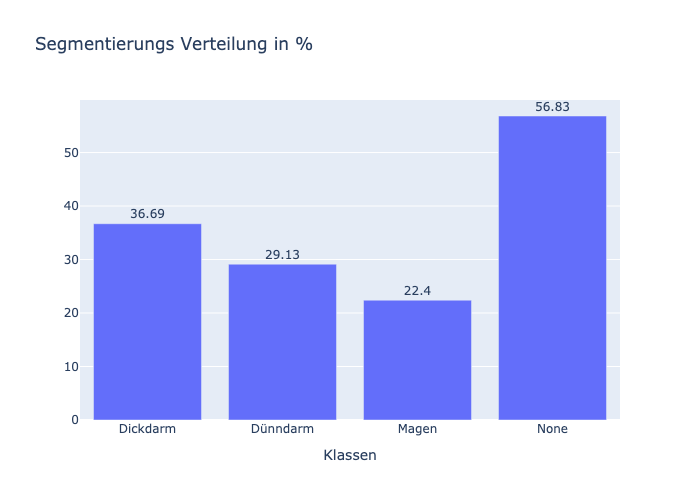
\includegraphics[width=220pt , angle=270]{bilder/segmentation_distribution}
		\caption{Verteilung der Klassen im Testset}\label{Fig:klassenverteilung}
	\end{center}
\end{figure}

\begin{figure}[!htb]
   \begin{minipage}{0.48\textwidth}
     \centering
     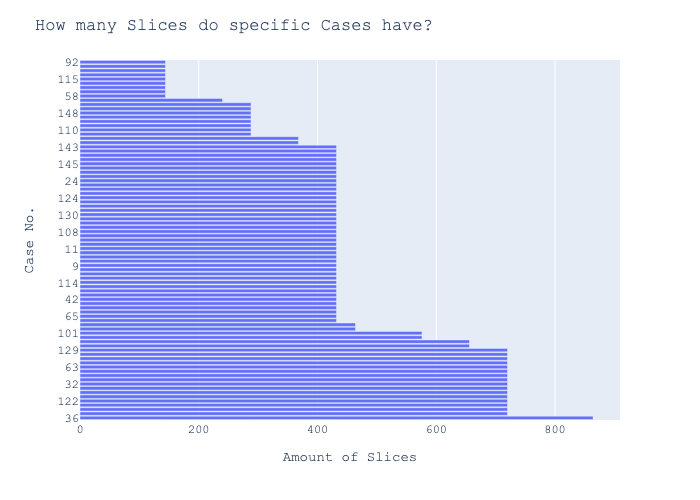
\includegraphics[width=1.2\linewidth]{bilder/slice_per_case}
     \caption{Anzahl Bilder pro Fall}\label{Fig:slice_per_case}
   \end{minipage}\hfill
   \begin{minipage}{0.48\textwidth}
     \centering
     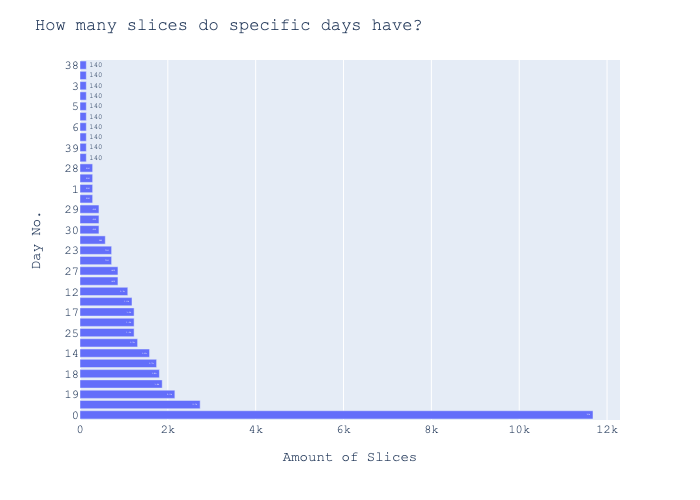
\includegraphics[width=1.2\linewidth]{bilder/slices_per_day}
     \caption{Anzahl Bilder pro Tag}\label{Fig:slice_per_day}
   \end{minipage}
\end{figure}

\subsection{Metadatenextraktion}

Anhand der ID eines jedes Slices war es möglich verschiedene Metadaten dem originalem Dataframe zu hinzuzufügen, zudem wurde die Gesamtlänge gedrittelt, dadurch dass die Klassen einer ID  zugewiesen worden sind, die Gesamtlänge des Dataframes beläuft sich somit auf 38 496 Zeilen. \autoref{tabelle_meta_daten}

% & rs & re & cs & ce & count & path00 & path01 & path02 & image\textunderscore paths

\begin{table}[H]
 \begin{center}
  \scalebox{0.7}{
   \begin{tabular}{|l|l|l|l|l|l|l|l|l|l|l|l|l|l|}
     \hline
     Idx  & ID &  large\textunderscore bowel & small\textunderscore bowel & stomach & case & day & slice & path & width & height & pixel\textunderscore x & pixel\textunderscore y \\
     \hline \hline
     1     & case134\textunderscore day0\textunderscore slice\textunderscore 0085 	& NaN & 41591 5  ...    & NaN & 134 & 0 & 85 & input\textbackslash  & 266 & 266 & 1.5 & 1.5  \\
     2     & case134\textunderscore day0\textunderscore slice\textunderscore 0086 	& 41591 27 ... & NaN    & NaN & 134 & 0 & 86 & input\textbackslash  & 266 & 266 & 1.5 & 1.5  \\
     3     & case134\textunderscore day0\textunderscore slice\textunderscore 0086 	& NaN & NaN   & NaN & 134 & 0 & 87 & input\textbackslash  & 266 & 266 & 1.5 & 1.5  \\
     \hline
   \end{tabular}
   }
   \caption{Metadaten von drei slices}\label{tabelle_meta_daten}
 \end{center}
\end{table}

\subsection{Vorarbeit}

\subsubsection{2.5 dimensionale Daten}

Klassisch haben die Slices die Dimensionen 
\begin{equation}
H \times W \times 1
\end{equation}
da es sich um graustufen Bilder handeln. U-Net arbeitet klassisch aber mit RGB Bildern, also einem 3 Channel Input
\begin{equation}
H \times W \times 3
\end{equation}
somit ist die Idee, aufeinanderfolgende Slices mit einem bestimmten Stride (Abstand) zu Verketten und dem Input so mehr Tiefe zu geben.

\begin{figure}[htb]
	\begin{center}
		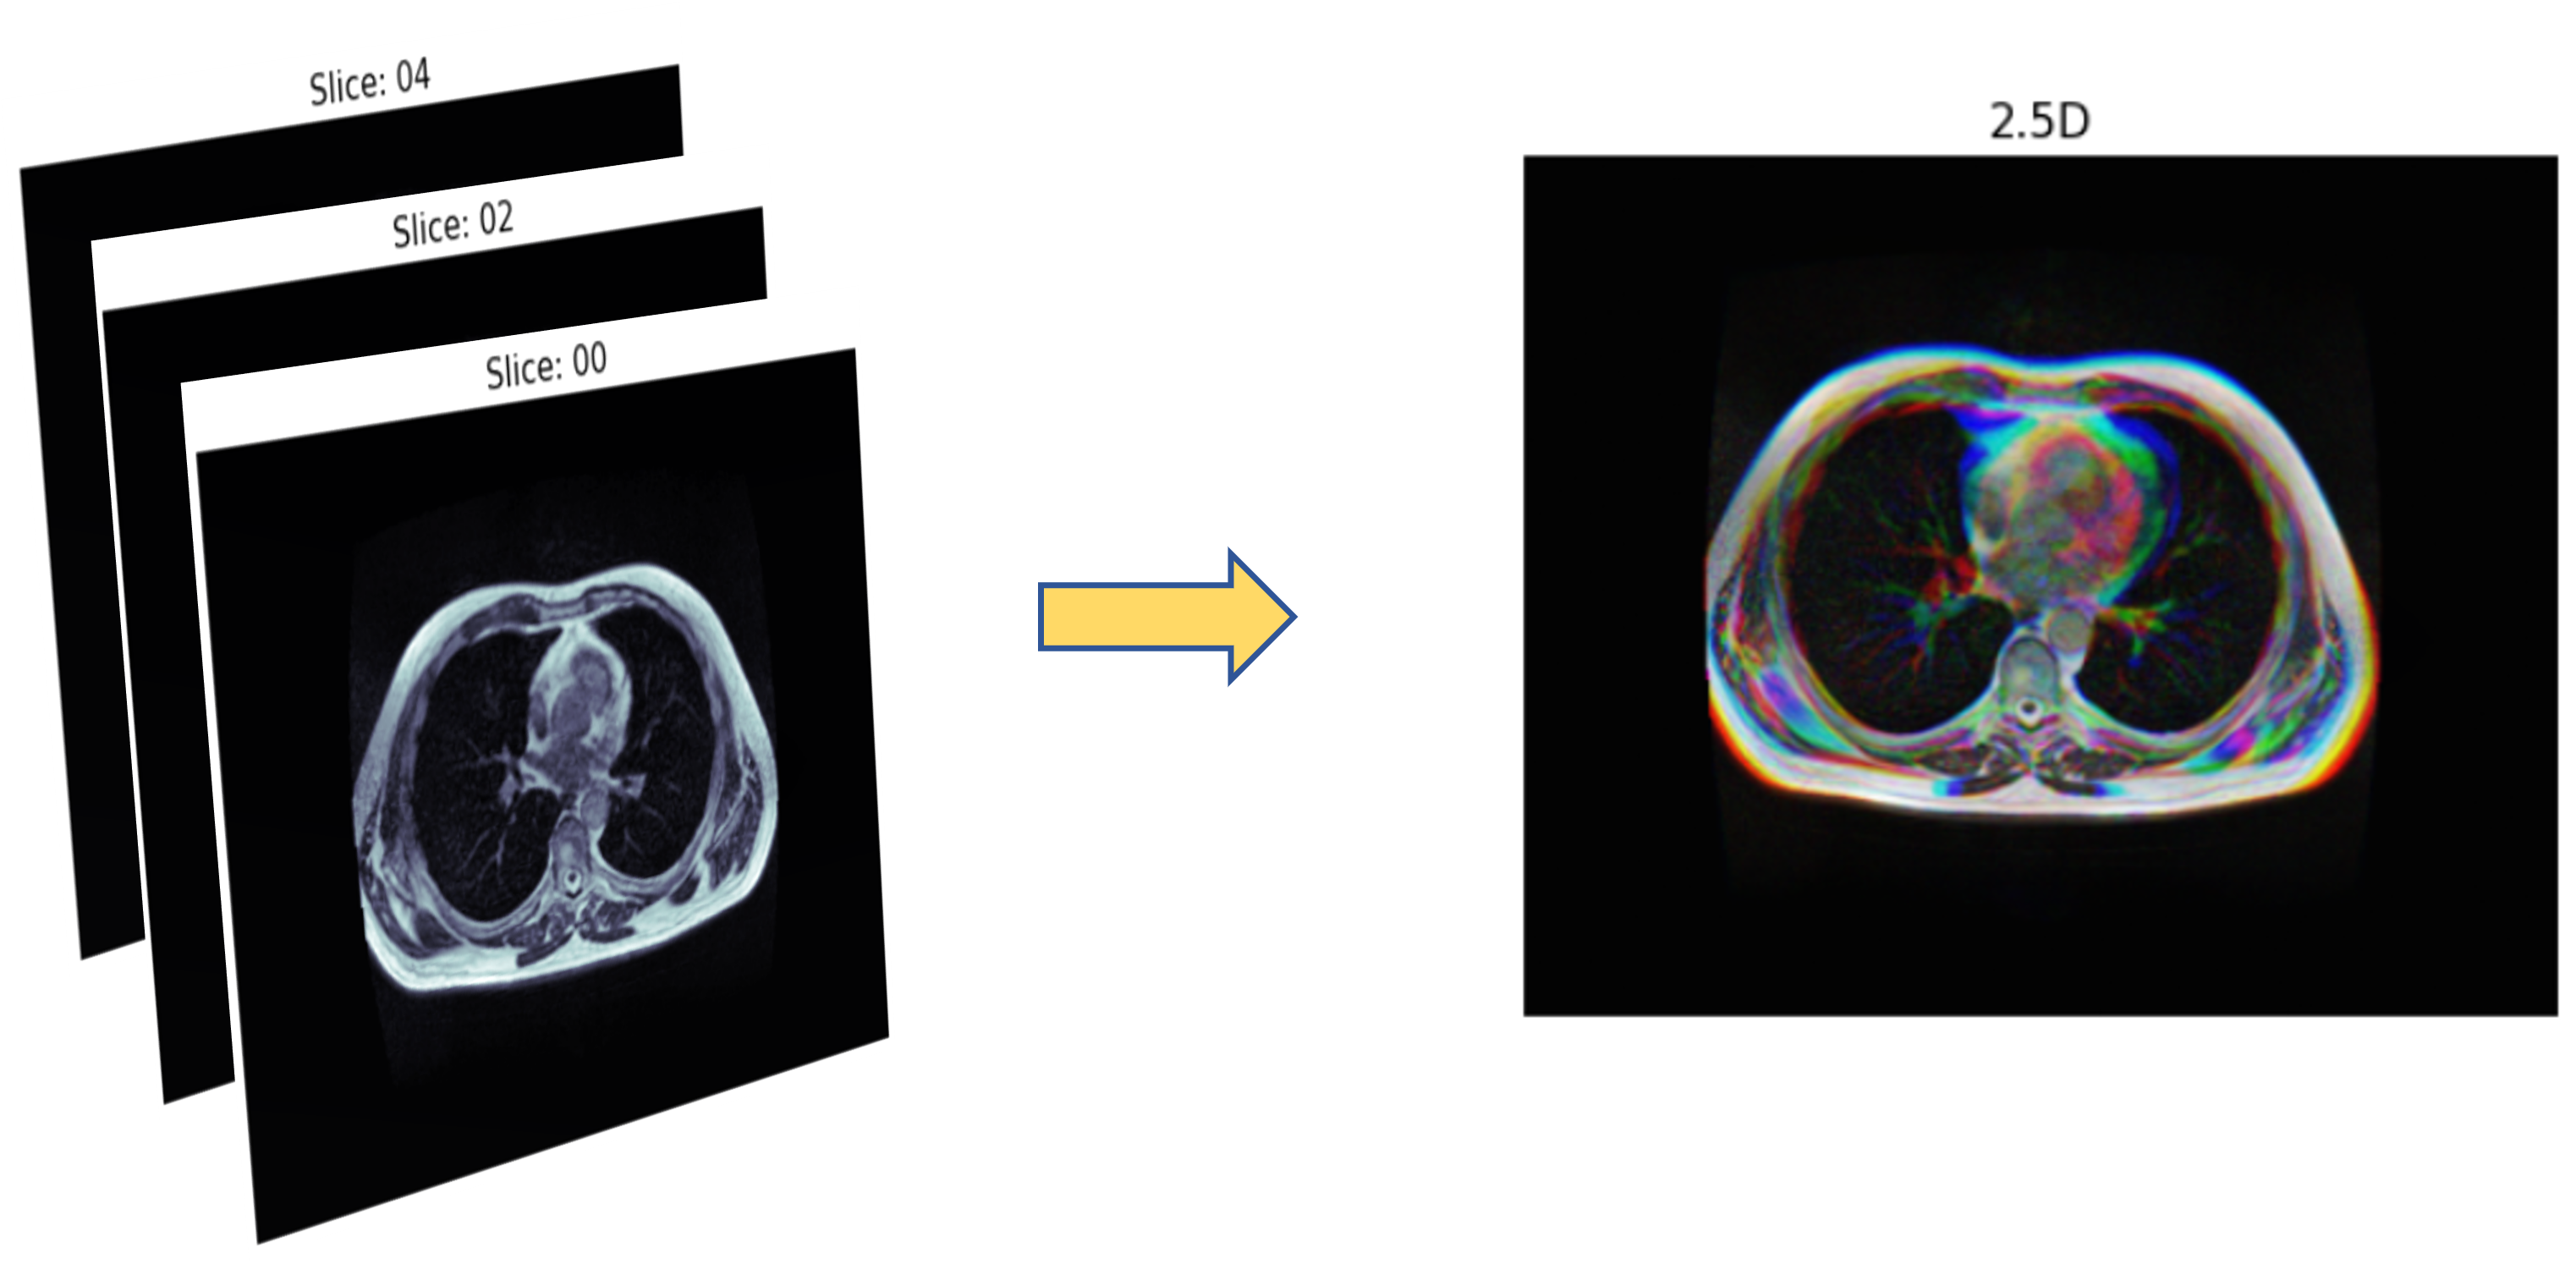
\includegraphics[width=450pt]{bilder/25d_input}
		\caption{Semi-3-dimensionaler Input}\label{Fig:25d-data}
	\end{center}
\end{figure}

Diese Methode hat gegenüber 3 dimensionalen Daten einige Vorteile: es wird weniger Rechenleistung benötigt, die Trainingspipeline muss nur minimal angepasst werden, die Auswertung bleibt ebenfalls gleich und die Daten können jedem Modell übergeben werden, welche darauf ausgelegt sind RGB Bilder zu segmentieren.

\subsubsection{Intelligentes Zuschneiden}

Basierend auf den Ergebnissen von Zaridis et al. sowie dem Vorhandensein eines Klassen-Ungleichgewichts implementierte ich einen Algorithmus, in der Hoffnung eine Verbesserung der Performance des Models zu erreichen.

Die Eingabebilder wurden für jeden Tag pro Case individuell zugeschnitten. Zu beginn wird das Hintergrundrauschen mit einem Medianfilter beseitigt, um das kleinste Rechteck aus der Menge zu finden, welches den Wertebereich enthält, der ungleich null ist. Dieser Prozess wird für jedes Slice aus dem Tag wiederholt, zum Schluss werden die Werte der Zeile angehangen, im Dataloader werden die Slices je nach Konfiguration dann zugeschnitten. Ein Beispiel von Case 134, Tag 21, Slice 70 ist hier zu sehen: \autoref{tab:crop_table} 

\begin{table}[H]
 \begin{center}
  \scalebox{1.1}{
\begin{tabular}{|l|l|l|l|l|l|l|}
\hline
 ID & Case & Day & RS & RE & CS & CE \\ \hline
 1 & 134 & 21 & 84 & 10000 & 0 & 359 \\ \hline
 2 & 113 & 22 & 50 & 10000 & 0 & 332  \\ \hline
\end{tabular}
}
\caption{Ausschnitt aus der Zuschnitt-Tabelle}\label{tab:crop_table}
 \end{center}
 \end{table}
 
 RS, RE, CS und CE stehen in diesem Kontext für Zeilenanfang und Ende sowie Spaltenanfang und Ende.
 
 So konnte das Ungleichgewicht für jede Klasse gesunken werden (Werte wurden gerundet): 

\begin{table}[H]
\centering
\begin{tabular}{l|c|c}
Klasse & ohne Zuschnitt & mit Zuschnitt \\ \hline
large\textunderscore bowel & 144 & 134\\
small\textunderscore bowel & 158 & 146 \\
stomach & 286 & 265\\
Total & 60 & 56\\
\end{tabular}
\caption{\label{tab:ratio}Verhältnis von Vorder- zu Hintergrundpixeln}
\end{table}


\begin{figure}[htp]
\centering
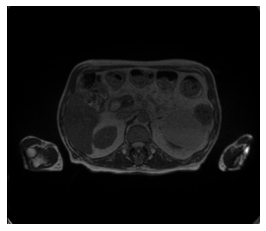
\includegraphics[width=.25\textwidth]{bilder/orig}\hfill
\caption{Original}
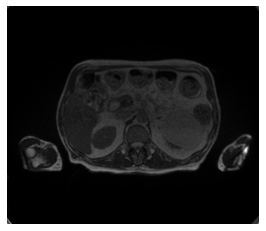
\includegraphics[width=.25\textwidth]{bilder/crop}\hfill
\caption{Zugeschnitten}
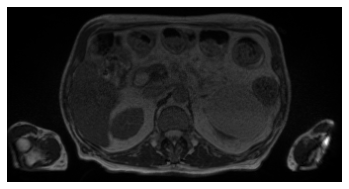
\includegraphics[width=.25\textwidth]{bilder/crop_median}
\caption{Zugeschnitten mit Medianfilter}
\label{fig:crop}
\end{figure}



\subsubsection{Bereinigen der Daten}

Zwei Cases wurden falsch annotiert und wurden deshalb aus dem Trainingsdatensatz entfernt, somit beläuft sich die Anzahl der Zeilen auf 38 208: \autoref{fig:cut}

\begin{figure}[htp]
\centering
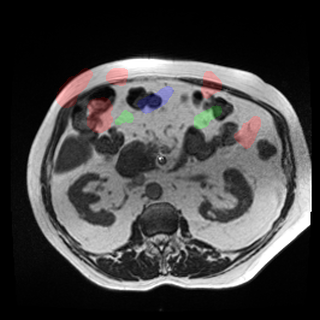
\includegraphics[width=.25\textwidth]{bilder/case7-day0-slice-0096}\hfill
\caption{Case 7, Tag 0, Slice 96}
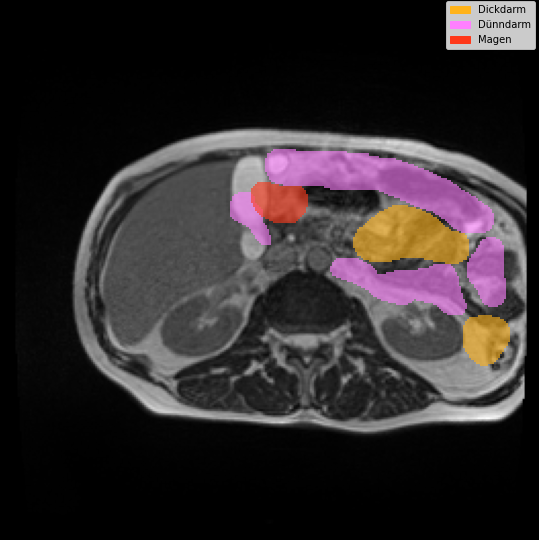
\includegraphics[width=.25\textwidth]{bilder/case81-day30-slice-0096}\hfill
\caption{Case 81, Tag 30, Slice 96}
\label{fig:cut}
\end{figure}

\subsection{Nacharbeit}

Bestimmte Slices weisen nie eine Segmentierung auf. Dieses Wissen kann man dazu nutzen, um die Vorhersage zu bereinigen, indem man die Maske jener Slices entfernt. Mithilfe dieser Methode kann man seinen Score bei Kaggle um e-3 bis e-4 verbessern. Ob dies jedoch good practice im Klinikalltag ist, ist fragwürdig, da diese Beobachtungen auf diesem Datensatz gemacht wurden und es wahrscheinlich ist aufgrund von z.B. einer anderen Statur, Operationen oder ähnlichem dies bei anderen Patienten nicht garantieren kann,

\subsection{Algorithmik}

\subsubsection{Hausdorff-Metrik} \label{ssec:hdorff}
Die Hausdorff-Metrik ist eine Methode zur Berechnung des Abstands zwischen den Segmentierungsobjekten X und Y, indem der am weitesten entfernte Punkt auf Objekt X vom nächstgelegenen Punkt auf Objekt Y berechnet wird

\begin{equation}
d_{\mathrm{H}}(X, Y)=\max \left\{\sup _{x \in X} d(x, Y), \sup _{y \in Y} d(X, y)\right\}
\end{equation}

\subsubsection{Binäre Kreuzentropie} \label{ssec:bce}

Die Kreuzentropie ist definiert als ein Maß für die Differenz zwischen zwei Wahrscheinlichkeitsverteilungen für eine bestimmte Zufallsvariable oder eine Reihe von Ereignissen. Sie eignet sich besonders gut Klassifizierungen auf Pixelebene, weist jedoch bei einer unausgewogenen Klassenverteilung der Daten ihre schwächen auf. \citep{Jadon_2020} 

Sie ist definiert als:
\begin{equation}
\mathcal{L}_{BCE}\left(X_{i l}, Y_{i} l\right)=\sum_{c=1}^{C} X_{i c l} \log \left(Y_{i c l}\right)
\end{equation}

\subsubsection{Dice-Koeffizient} \label{ssec:dc}

Der Dice-Koeffizient kann verwendet werden, um die pixelweise Übereinstimmung zwischen einer vorhergesagten Segmentierung und der entsprechenden Groundtruth zu vergleichen. Die Formel ist gegeben durch:

\begin{equation}
D S C=\frac{2|X \cap Y|}{|X|+|Y|}
\end{equation}

wobei X die vorhergesagte Menge von Pixeln und Y die Groundtruth ist. Der Dice-Koeffizient ist definiert als 0, wenn sowohl X als auch Y leer sind.

\subsection{Modell}

Das Projekt wurde gänzlich in Python mithilfe der TensorFlow API sowie dem
 \href{https://deepai.org/machine-learning-glossary-and-terms/relu}{Segmentation Models} \citep{Yakubovskiy:2019}
 Package aufgezogen, welches verschiedene Architekturen inklusive an- und nicht antrainierte Encoder zur verfügung stellt. 
 
 Trainiert wurde mit dem
\href{https://optimization.cbe.cornell.edu/index.php?title=Adam}{Adam Optimizer},
 und einer initialen Learning Rate von von 5e-4, die sich um den Faktor e-1 verringert, wenn der Validation-loss nach fünf Epochen unverändert schlecht blieb. 
 
 Die Loss function ist eine Mischung aus 
\href{https://www.analyticsvidhya.com/blog/2021/03/binary-cross-entropy-log-loss-for-binary-classification/}{Binary Crossentropy} und zu einem Faktor von 0.5 der Dice-Koeffizient. Diese Kombination eignet sich laut Jadon  \citep{Jadon_2020} besonders gut, um einen höheren Dice Score zu erzielen. Außerdem ermöglicht sie dem Modell, sich auf mehrere Klassen zu konzentrieren, so ist das Modell in der Lage das Klassenungleichgewicht zu berücksichtigen. 

\begin{equation}
\mathcal{L}\left(X_{i l},{Y_{i}} l\right)= 0.6 * \sum_{c=1}^{C} X_{i c l} \log \left({Y}_{i c l}\right)+0.4 *\left(1-\frac{2\left|X_{i l} \cap {Y_{i}} l\right|}{\left|X_{i l}\right|+\left|{Y_{i}} l\right|}\right)
\end{equation}

Es wurde mit einer Batchsize von 16 und 32 auf verschiedenen Grafikkarten vom 
\href{https://wiki.hhu.de/display/HPC/Abschlussarbeiten+im+HPC}{HPC} des ZIMs Trainiert: RTX 8000, RTX 6000 und GTX 1080ti.

Die Daten wurden mithilfe von der 
\href{https://scikit-learn.org/stable/modules/generated/sklearn.model_selection.StratifiedGroupKFold.html}{StratifiedGroupKFold} Methode von Sklearn in 5 Folds aufgeteilt nach Case gruppiert mit einem festem Seed von 42. Somit wurde das Verhältnis der Klassendistribution im Vergleich zum ganzen Datensatz in jedem Fold beibehalten. 

\subsection{Experimente}
Zunächst wurde eine Baseline mit folgenden Standardkonfigurationen geschaffen:

\begin{table}[H]
\centering
\begin{tabular}{l|c|c|c}
Input & Batchsize & Epochen & Datenbereinigung \\\hline
256x256x1 & 16 & 50 & Wahr \\
\end{tabular}
\caption{\label{tab:widgets}Baseline Einstellungen}
\end{table}

Zunächst wurden mit diesen Konfigurationen 12 verschiedene Modelle trainiert, wessen Encoder auf
\href{https://www.image-net.org/}{ImageNet} angelernt wurden.

\begin{table}[H]
\resizebox{\textwidth}{!}{\begin{tabular}{l|c|c|c|c|c|c|c|c|c}
Encoder & Beste Epoche &      Loss & Val. loss & Dice  & Val. Dice  & IoU & Val. IoU & Privat & Öffentl. \\\hline
efficientnetb7 &           14 & 0.0500 &    {\bf 0.1064} & 0.8848 &    {\bf 0.7636} & 0.8153 &   0.8223 & 0.8293 & {\bf 0.8467}  \\
efficientnetb2 &           22 & 0.0369 &    0.1123 & 0.9146 &    0.7489 & 0.9037 &   0.8195 & 0.8278 &  0.8434\\
efficientnetb1 &           18 & 0.0425 &    0.1158 & 0.9018 &    0.7386 & 0.8889 &   0.8179  & 0.8266 & 0.8416  \\
efficientnetb5 &           25 & 0.0369 &    0.1160 & 0.9146 &    0.7378 & 0.9089 &   0.8161 & 0.8315 & 0.8457  \\
   inceptionv3 &           30 & 0.0381 &    0.1186 & 0.9118 &    0.7326 & 0.8937 &   0.8108  & 0.8201 & 0.8385  \\
efficientnetb3 &           22 & 0.0382 &    0.1181 & 0.9117 &    0.7324 & 0.8958 &   0.8206 & 0.8235 & 0.8434  \\
   densenet121 &           33 & 0.0385 &    0.1198 & 0.9109 &    0.7300 & 0.8873 &   0.8093 & 0.8179 & 0.8346  \\
efficientnetb6 &           19 & 0.0401 &    0.1194 & 0.9073 &    0.7277 & 0.8925 &   {\bf 0.8240} & {\bf 0.8357} & 0.8463 \\
efficientnetb4 &           35 & {\bf 0.0317} &    0.1211 & {\bf 0.9267} &    0.7266 & 0.9235 &   0.8147 & 0.8243 & 0.8426  \\
      resnet50 &           35 & 0.0324 &    0.1244 & 0.9250 &    0.7206 & {\bf 0.9259} &   0.7974  & 0.8081 & 0.8278 \\
   densenet201 &           43 & 0.0383 &    0.1553 & 0.9114 &    0.6406 & 0.8942 &   0.7893 & 0.8176 & 0.8322  \\
efficientnetb0 &           21 & 0.0387 &    0.1641 & 0.9104 &    0.6173 & 0.8804 &   0.7864 & 0.8227 & 0.8406  \\
\end{tabular}}
\caption{\label{tab:baselines}Baseline Performances nach Validation loss absteigend sortiert.}
\end{table}

Hier sticht efficientnetb7 klar hervor mit großem Abstand, wenn man den Validation loss betrachtet. 

-> iou score für predictions vom validation set berechnen und beste + schlechteste masken plotten + score bei kaggle 

-> efb2 und dense121 

-> die werden erneut trainiert mit bereinigten Daten, 25D Daten und / oder zugeschnittenen Daten

-> inputsize erhöht

-> iou score für predictions vom validation set berechnen und beste + schlechteste masken plotten + score bei kaggle 

-> was hat wo was gebracht (25d daten, zuschnitt, datenreinigung) 

\section{Evaluation}\raggedbottom

\section{Fazit}\raggedbottom

\subsection{Ausblick}
Ideen, die es nicht in die Arbeit geschafft haben oder nicht schafffen konnten.

\ifthenelse{\equal{\sprache}{deutsch}}{
	\textbf{quotes}:\\
	Ein Beispiel für deutsche Anführungszeichen \glqq quote\grqq.
}{}

\pagebreak
